%!TEX root=../../../main.tex

Kravet til pH-proben er at den skal virke omgående når der hældes gødning i vandet. Dette vil sige at den løbende skal kunne informere systemet når der er den korrekte pH-værdi, under dosering af gødning. Efter nogle søgninger på Google blev der fundet frem til, at en glasprobe var den mest effektive, og samtidig også den billigste løsning. 

\begin{figure}[H]
	\centering 
	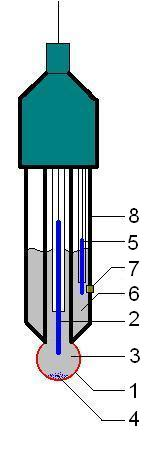
\includegraphics[scale=0.7]{HardwareArkitektur/Sensore/pH_probe_billeder/Glass_electrode_wiki.jpg}
	\caption{Tegning af en glasprobe. kilde: Wikipedia}
	\label{photo:pH-probe}
\end{figure}     

pH-værdi er en måde at angive hvor mange hydrogen-ioner der er i en given væske. Definitionen af en syre, er at den modtager hydrogen-ionerne, og definitionen af en base er at den afgiver hydrogen-ioner. Vand kan både optræde som en syre og en base, dette skyldes, at vand vil modtage hydrogen-ionerne når der blandes base i, og afgive hydrogen-ioner når der blandes syre i. På fig. \ref{photo:pH-skala} ses at hvis der findes $10^{-14}$ mol/l af H+ ioner, ligger pH-værdien på 14. 

 \begin{figure}[H]
	\centering 
	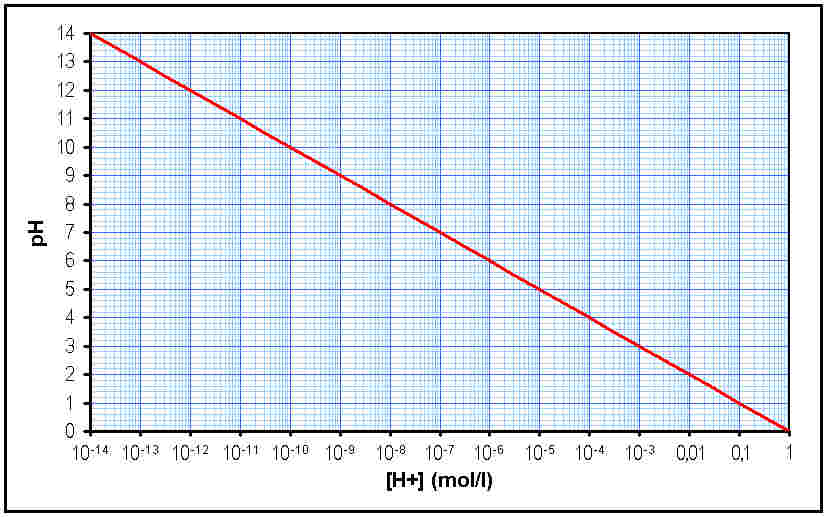
\includegraphics[scale=0.4]{HardwareArkitektur/Sensore/pH_probe_billeder/PH-skala.jpg}
	\caption{Graf over pH-værdi. kilde: Wikipedia}
	\label{photo:pH-skala}
\end{figure}   

Glasproben virker ved at at den, internt er fyldt op med saltsyre HCL. På fig.\ref{photo:pH-probe} punkt 3 er koncentrationen $1*10^{-7}$ mol/l. I punkt 6 er koncentrationen $0.1$ mol/l. På denne måde bliver der genereret en spænding når der er overskud eller underskud af H+ ioner på ydersiden af punkt 1. H+ ionerne vil tiltrække CL-ionerne som ses i punkt 4. Punkt 2 og 5 er elektroderne som der måles spændingen over. På fig.\ref{photo:probeslope} ses outputtet fra proben i forhold til pH-værdien af den væske den befinder sig i. 

 \begin{figure}[H]
	\centering 
	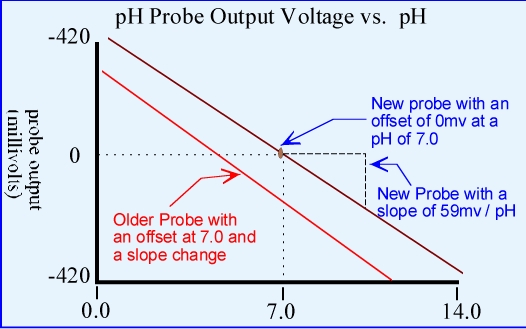
\includegraphics[scale=0.4]{HardwareArkitektur/Sensore/pH_probe_billeder/probeslope.jpg}
	\caption{Outputtet fra pH-proben}
	\label{photo:probeslope}
\end{figure} 

For at få en præcis måling af væsken kræver det at der laves en kalibrering af pH-proben én gang hver måned. Dette skyldes at proben vil drift'e med tiden. Det ses også på fig.\ref{photo:probeslope} at en ny probe vil give en højere spænding end en ældre probe. Til kalibrering af proben skal der anvendes en buffervæske. Buffervæske er en væske med en præcis pH-værdi således at proben kan indstilles efter det. Måden dette gøres på er at benytte en buffer med pH-værdi 7. Når systemet startes op skal proben kalibreres og der vil her være en rød LED på karet der lyser. For at kalibrere proben sættes den ned i buffervæsken, og efter ca. 30 sekunder trykkes der på kalibrerings-knappen som sidder på karet og værdien indlæses herved. På fig.\ref{photo:buffer_vaeske} ses at buffervæsken varierer sin pH-værdi ved forskel temperatur. Dette vil også være gældende for andre væsker, dog er dette ikke noget der tages højde for i disse målinger, men dette bør implementeres i et salgsklart system. 

 \begin{figure}[H]
	\centering 
	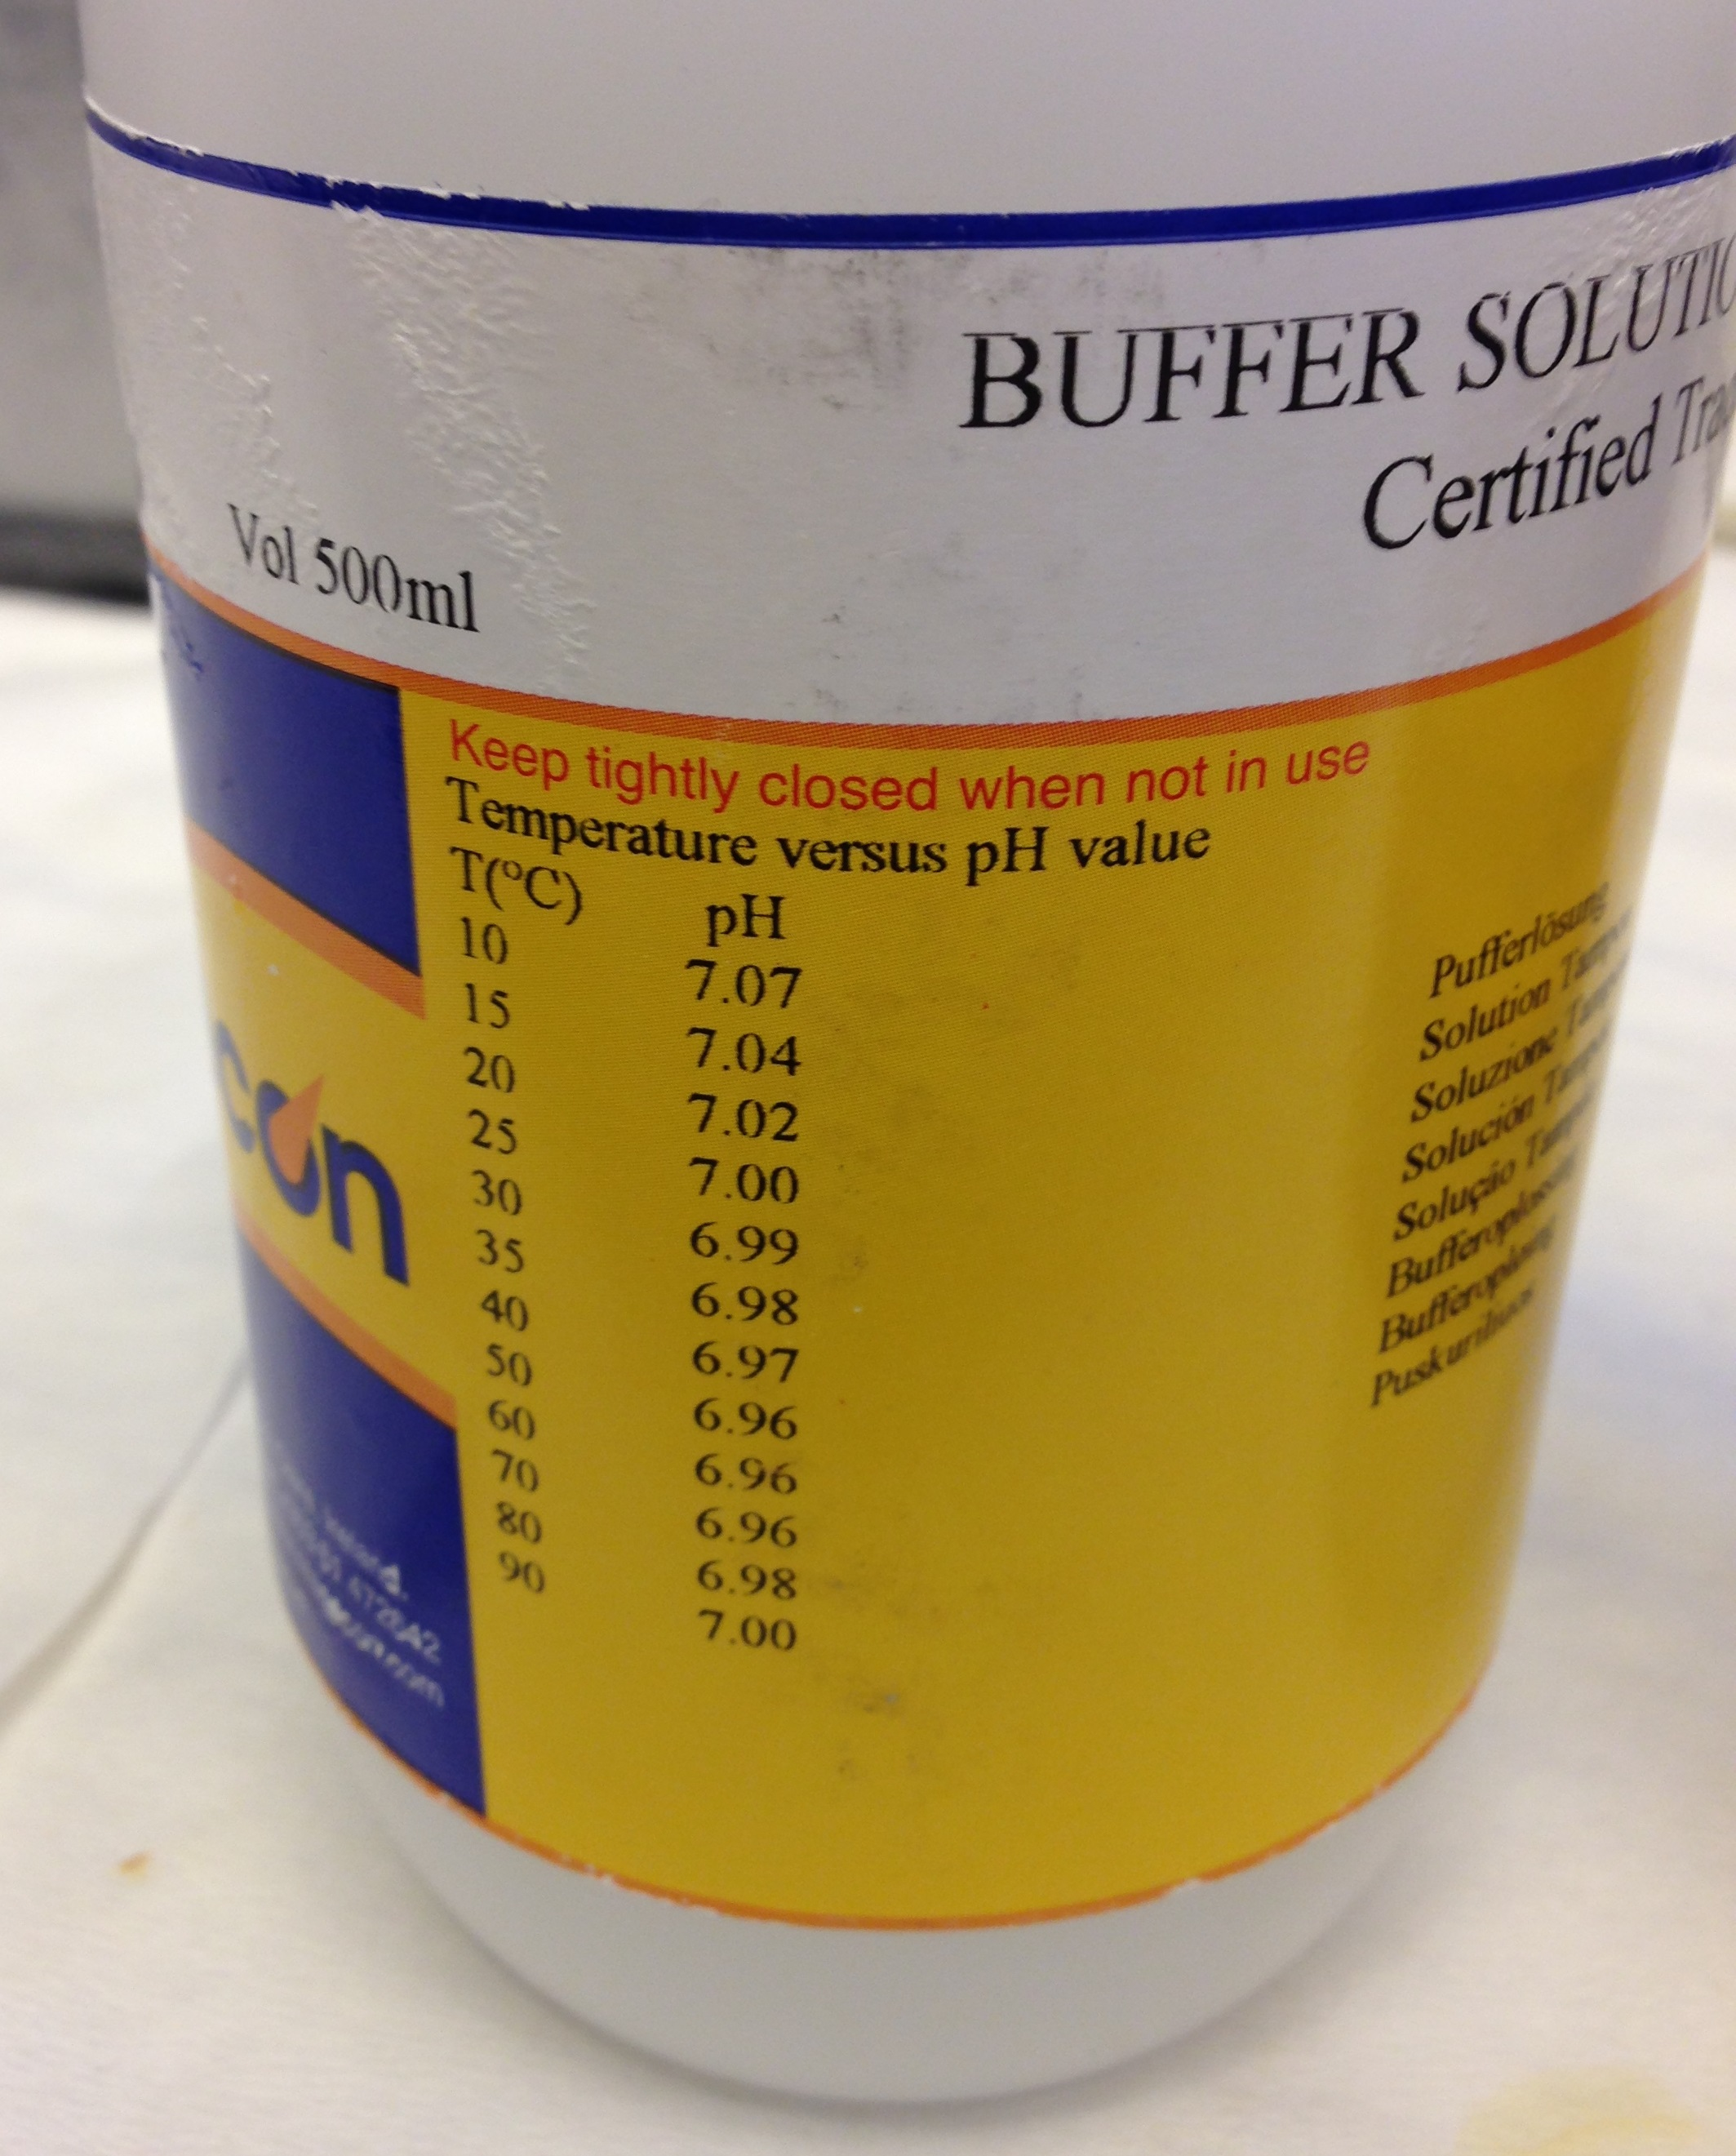
\includegraphics[scale=0.1]{HardwareArkitektur/Sensore/pH_probe_billeder/buffervaeske.jpg}
	\caption{Temperaturens indflydelse på pH-værdien i buffervæsken}
	\label{photo:buffer_vaeske}
\end{figure} 
Nedenfor ses koden til pH-proben-software'en. Koden er herefter klar til at blive implementeret i kar-softwaren. For overskuelighedens skyld vælges det at vise den individuelle kode her. Der er oprettet en funktion getPhVal() som returnerer pH-værdien.

\lstinputlisting[language=c]{HardwareArkitektur/Sensore/Kode/pH_kode.c} 

\subsection{Støj}

For at få en præcis måling analyseres proben for dens egenstøj. Dette gøres ved at lave et nyt PSoC projekt. I Mixed Signal Electronic's har vi arbejdet med dette og herfra kopieres derfor et følgende kredsløb. Det skal dog siges at projektet er til PSoC5 og her i Projektet benyttes en PSoC4. PSoC5 har den fordel at den har en DeltaSigma ADC som er bedre til at sample lavfrekvente signaler. I PSoC4 er den eneste mulighed en SAR-konverter. På fig.\ref{photo:Topdesign_stoj} ses topdesignet i PSoC Creator. 
 \begin{figure}[H]
	\centering 
	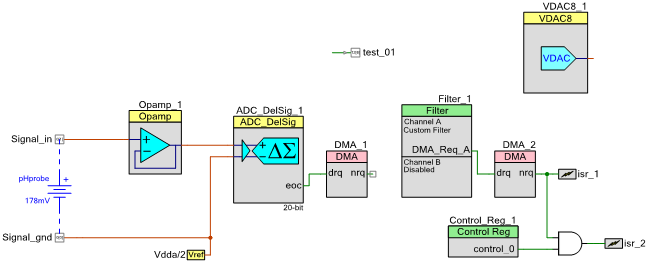
\includegraphics[scale=0.8]{HardwareArkitektur/Sensore/pH_probe_billeder/Topdesign_stoj.png}
	\caption{Topdesign i PSoC creator over kredsløbet til støjmåling}
	\label{photo:Topdesign_stoj}
\end{figure} 

For at kunne beregne støjen fra proben måles dens indre modstang og derefter benytte Johnson Nyquist formel for termisk støj. 
$$ V_n = \sqrt{4*K*T*R*\Delta f} $$

For at måle den indre modstand i proben kobles den med en buffer i PSoC4. Det blev forsøgt at måle selve indgangsimpedansen i bufferen da denne ikke var opgivet i databladet. Dette var desværre ikke muligt da støj på indgangen fik den til at klippe på udgangen. Det antages derfor at indgangsimpedansen er uendelig stor, for at måle udgangsspændingen ubelastet opstilles kredsløbet som ses på fig.\ref{photo:Non_inv_buf}. 

 \begin{figure}[H]
	\centering 
	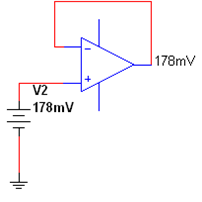
\includegraphics[scale=1]{HardwareArkitektur/Sensore/pH_probe_billeder/Non_inverting_buffer.png}
	\caption{Non-inverting buffer}
	\label{photo:Non_inv_buf}
\end{figure} 

Der måltes 178mV over udgangen af bufferen med proben sat ned i buffervæske med en pH-værdi på 4. Derefter blev proben sat direkte i oscilloskopet som har en indgangsimpedans på 1M\ohm . Nedenstående kredsløb opstilles for denne måling, fig. \ref{photo:Kredslob_RI}. 


 \begin{figure}[H]
	\centering 
	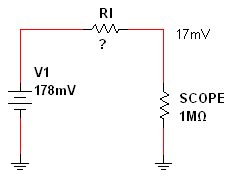
\includegraphics[scale=1]{HardwareArkitektur/Sensore/pH_probe_billeder/Kredslob_RI.png}
	\caption{Diagram over den indre modstand}
	\label{photo:Kredslob_RI}
\end{figure} 

Med Ohms-lov beregnes den indre modstand til at være 9.5M\ohm . Derfor beregnes støjbidraget til at være
$$ V_n = \sqrt{4*1.3806488*10^{-23}*297*9.5*10^{6}*100} = 3.9uV $$.
Selve bufferen har også et støjstrøms bidrag som vil resultere i en støjspænding over modstanden i proben. I MSE øvelse 5 blev der arbejdet med disse støjstrømme og der kan med viden herfra antages at bufferen bidrager med $5pA$ i støjstrøm. I PSoC'en benyttes et digitalt filter på 100Hz. Optimalt set have fc været på 1Hz, men det mindste det lykkedes at implementere var fc = 100Hz.
$$ V_n = I_{rms}*R_i*\sqrt{\Delta f} = 5pA*9.5M\ohm *\sqrt{100} = 475uV $$
Støj fra bufferen:
$$ V_n = 1.3uV * \sqrt{100} = 13uV $$
Støj fra ADC'en:
$$ V_n = 10uV * \sqrt{100} = 100uV $$
For at addere støjbidragene adderes disse kvadratisk da de udregnes støj er RMS-værdier:
$$ V_{ntot} = \sqrt{3.9uV^2 + 475uV^2 + 13uV^2 + 100uV^2} = 485uV $$
Det ses at det største og mest betydende støjbidrag er støjstrømmen fra bufferen.\newline 

\subsubsection{Måling af støj}

For at måle støjen åbnes TeraTerm og udlæser værdien. I projektet er der lavet funktioner til at udskrive støjværdierne over UART. Proben sættes nu i en buffervæske med pH-værdi = 4. På fig.\ref{photo:stoj_teraterm} ses måling af den samlede støj på ca 4.8mV.

 \begin{figure}[H]
	\centering 
	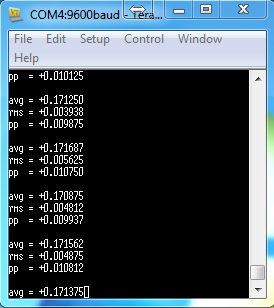
\includegraphics[scale=1]{HardwareArkitektur/Sensore/pH_probe_billeder/stoj_teraterm.png}
	\caption{Udlæsning på teraterm}
	\label{photo:stoj_teraterm}
\end{figure} 

 \begin{figure}[H]
	\centering 
	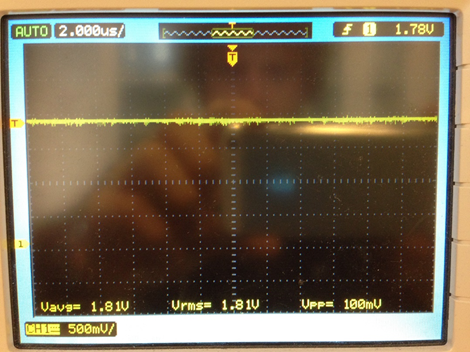
\includegraphics[scale=0.9]{HardwareArkitektur/Sensore/pH_probe_billeder/stoj_oscilloscope.png}
	\caption{Måling fra DAC'en på scopet}
	\label{photo:stoj_scope}
\end{figure} 

\subsubsection{Responstid}
For at måle responstiden, sættes proben i buffer 7 og derefter direkte over i buffer 4. Da H+ ionerne stadig vil sidde på proben når den trækkes op af buffer 7, sker der først en reaktion når den kommer i kontakt med buffer 4. Denne respons ses på fig. \ref{photo:respons}. Her aflæses responstiden til 1.4 sekunder.

 \begin{figure}[H]
	\centering 
	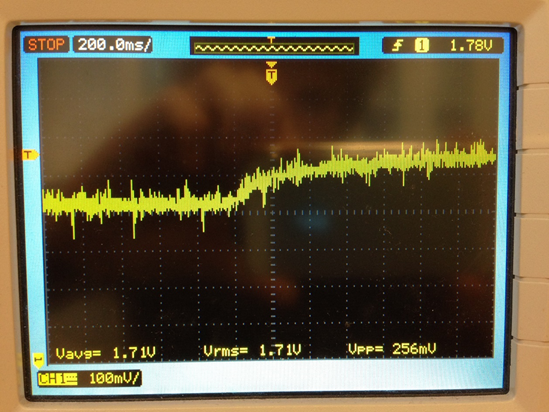
\includegraphics[scale=0.8]{HardwareArkitektur/Sensore/pH_probe_billeder/respons.png}
	\caption{Responstiden fra proben}
	\label{photo:respons}
\end{figure} 

\subsubsection{Probens præcision}
Selve proben vil have en måleafvigelse. Denne afvigelse tages der tildels højde for ved kalibreringen, men dette er kun den systematiske fejl der bliver reguleret ind. Der vil også være et antal tilfældige fejl, som vil være umulige at justere ind. For at få et overblik over fejlprocenten udføres der 10 målinger efter kalibrering af buffer 7. Her sættes proben ned i en kop vand, for derefter at sætte den ned i pH-bufferen igen. Der ventes i 2 minutter og pH-værdien aflæses herefter i debugging-mode.\newline Målingerne indskrives i et excel-dokument således at der kan udregne standardafvigelsen ved en konfidens på 95. Det skal dog siges at dette er en meget simplificeret metode, da der her ikke taget højde for temperaturforskelle. Der udføres også kun 10 målinger ved en bestemt pH-værdi. Der burde udføres målinger over hele aksen, for at afdække hele måleusikkerheden.    

 \begin{figure}[H]
	\centering 
	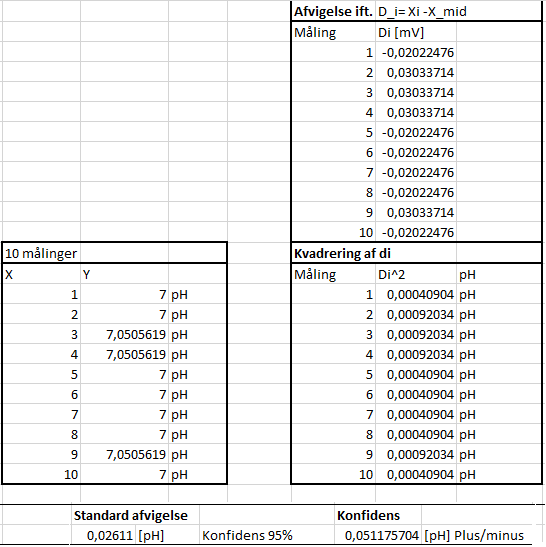
\includegraphics[scale=1]{HardwareArkitektur/Sensore/pH_probe_billeder/Probe_afvigelse.PNG}
	\caption{Probens præcision}
	\label{photo:probe_afvigelse}
\end{figure} 

Det ses at vi med 95\% sikkerhed kan sige at den målte værdi ligger inden for +-0,051175704 i pH-værdi, men som nævnt tidligere er dette ikke en endelig præcision.    

\subsubsection{Fremtidigt arbejde}
Vi så i denne del at vores beregnede støj var ca en faktor 10 større ved realiseringen end beregningerne. Dette kan skyldes at der er støj i tilledningerne da vi arbejder med ekstremt høje impedanser. Vi kan hermed konkludere at ved meget høje impedanser bliver ens udstyr meget støjfølsomt og det er derfor vigtigt at tage det med i beregningerne når der udlægges print, samt ved beslutning om hvilken terminering der skal benyttes. Fremtidigt arbejde kan være at lave kalibreringsfunktionen således den selv giver besked, når der er gået en måned, om at det er tid til kalibrering. 



